\iffalse
\chapter{Testarea aplicației și rezultate experimentale}
\label{cap:cap4}

(cel puțin 5 pagini)

\begin{itemize}
    \item Punerea în funcțiune/lansarea aplicației,elemente de configurare sau instalare;
    \item Testarea sistemului (hardware/software);
    \item Aspecte legate de încărcarea procesorului, memoriei, limitări în ce privește transmisia datelor/comunicarea;
    \item Se prezintă datele de test/metrici/benchmarks
    \item Aspecte legate de fiabilitate/securitate;
    \item Rezultate experimentale;
    \item Utilizarea sistemului. 
\end{itemize}

\vspace{2cm}

\section{Nivel 1}
\label{cap:cap4:nivel1}

\textcolor{gray}{\lipsum}  (Figura \ref{fig:clone_trooper})

\begin{figure}[H]
    \centering
    
\includegraphics[width=0.3\textwidth]{continut/capitol4/figuri/clone_trooper.png}
    \caption{Clone Trooper\protect\footnotemark}
    \label{fig:clone_trooper}
\end{figure}
\footnotetext{imagine preluată de pe un site web care nu „merită” trecut la bibliografie \url{https://www.pngitem.com/}}

Tabelul \ref{tabel:tab_simplu} prezintă un exemplu foarte simplu de tabel în \LaTeX. Un alt exemplu este prezentat în Tabelul \ref{tabel:2} din \ref{anexa3:func_xyz}.

\begin{table}[ht]
    \centering
    \caption{Exemplu de tabel simplu}
    \label{tabel:tab_simplu}
    \begin{tabular}{||c l c r||} 
        \hline
        \textbf{Col1} & \textbf{Col2} & \textbf{Col3} & \textbf{Col4} \\
        \hline\hline
        1 & 6 & 87837 & 787 \\ 
        2 & 7 & 78 & 5415 \\
        3 & 545 & 778 & 7507 \\
        4 & 545 & 18744 & 7560 \\
        5 & 88 & 788 & 6344 \\
        \hline
    \end{tabular}
\end{table}

\subsection{Nivel 2}
\label{cap:cap4:nivel1:nivel2}

\subsubsection{Nivel 3}
\label{cap:cap4:nivel1:nivel2:nivel3}

\textcolor{gray}{\lipsum}

\textcolor{gray}{\lipsum}

\textcolor{gray}{\lipsum}

\fi

\chapter{Rezultatele experimentale}
\label{cap:cap4}

\section{Măsurători de performanță}

Din păcate, datorită unei schimbări de ultim moment în infrastructura cloud de la IBM Quantum Experience, două calculatoare cuantice de 5 biți (inclusiv IBMQ\_Bogota, cel folosit inițial de mine) au fost scoase, fiind înlocuite cu două calculatoare pe 7 biți. Deși acest lucru este un lucru bun, înseamnă de asemenea că timpul de stat la coadă (queue time) pentru acces la calculatoarele cuantice a crescut foarte mult, datorită entuziasmului din partea comunității pentru acces la calculatoare cu mai mulți qubiți. Acest lucru a făcut aproape imposibilă măsurarea performanțelor pe calculatoare cuantice adevărate, fiindcă pentru a obține niște măsurători exacte, algoritmul trebuie rulat de câteva ori, ori pentru fiecare acces la calculatorul cuantic, trebuie așteptat 20-25 de minute, făcând acest lucru o imposibilitate practică. 

\begin{figure}[H]
    \centering
    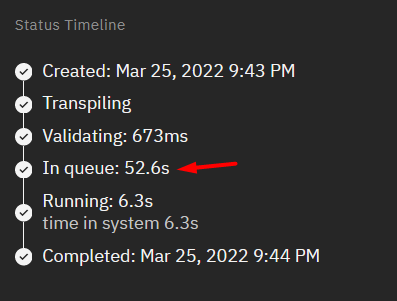
\includegraphics[width=1.0\textwidth]{continut/capitol4/figuri/WaitTime1.png}
    \caption{Timpul de așteptare pentru calculatorul cuantic IBMQ\_Bogota, folosit inițial}
    \label{fig:WaitTime1}
\end{figure}

\begin{figure}[H]
    \centering
    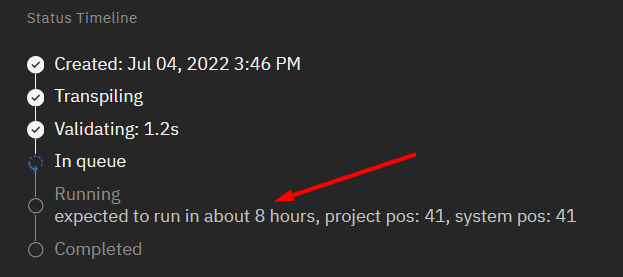
\includegraphics[width=1.0\textwidth]{continut/capitol4/figuri/WaitTime2.png}
    \caption{Timpul de așteptare pentru cel mai puțin ocupat calculator cuantic, în data de 4 iulie}
    \label{fig:WaitTime2}
\end{figure}

\subsection{Timpi de execuție pentru generatoarele de numere aleatorii uniforme}

În figura următoare sunt prezentați timpii de execuție pentru 100 de rulări a tuturor algoritmilor de generare a distribuțiilor uniforme (atât cuantice, cât și clasice), acestea generând 100000 de numere pentru fiecare experiment. Convențional, am ales începutul măsurătorii de timp ca începutul funcției de generare a numerelor și finalul ca momentul în care vectorul care conține toate cele 100000 de numere devine disponibil programatorului.

\begin{figure}[H]
    \centering
    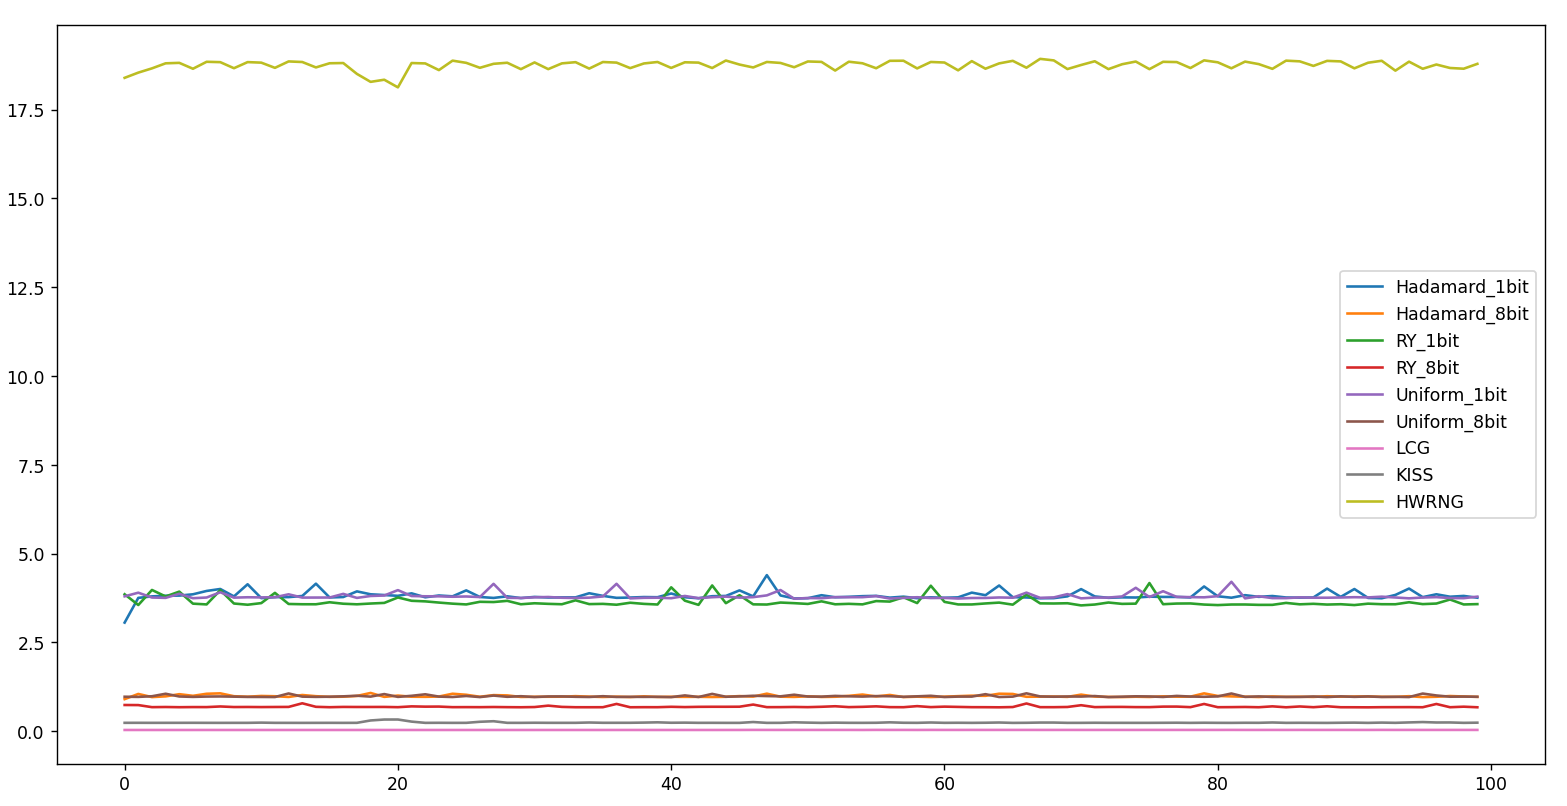
\includegraphics[width=1.0\textwidth]{continut/capitol4/figuri/PerformancesUniform.png}
    \caption{Timpii de execuție pentru generatoarele pe distribuție uniformă}
    \label{fig:UniformPerformances}
\end{figure}

Motivul pentru care generatorul de numere aleatorii hardware pare a fi atât de neperformant sunt diferențele de specificații dintre cele două laptopuri descrise în \ref{fig:BenchmarkLenovo} și \ref{fig:BenchmarkMyria}. Scalând rezultatele pentru HWRNG după performanță (cu un factor de 365/922 = 0.396), ținând rezultatele pentru celelalte generatoare pe loc, se obține un timp mediu de executie $17.7 \longrightarrow 7.009$. Chiar și așa, semnificativ mai încet decât timpii de execuție pentru celelalte generatoare, posibil datorită overhead-ului impus de lucru cu kernel-ul Linux.

Mediile timpilor de execuție pentru cele 100 de experimente, după scalarea coloanei HWRNG, sunt prezentate în figura următoare:

\begin{figure}[H]
    \centering
    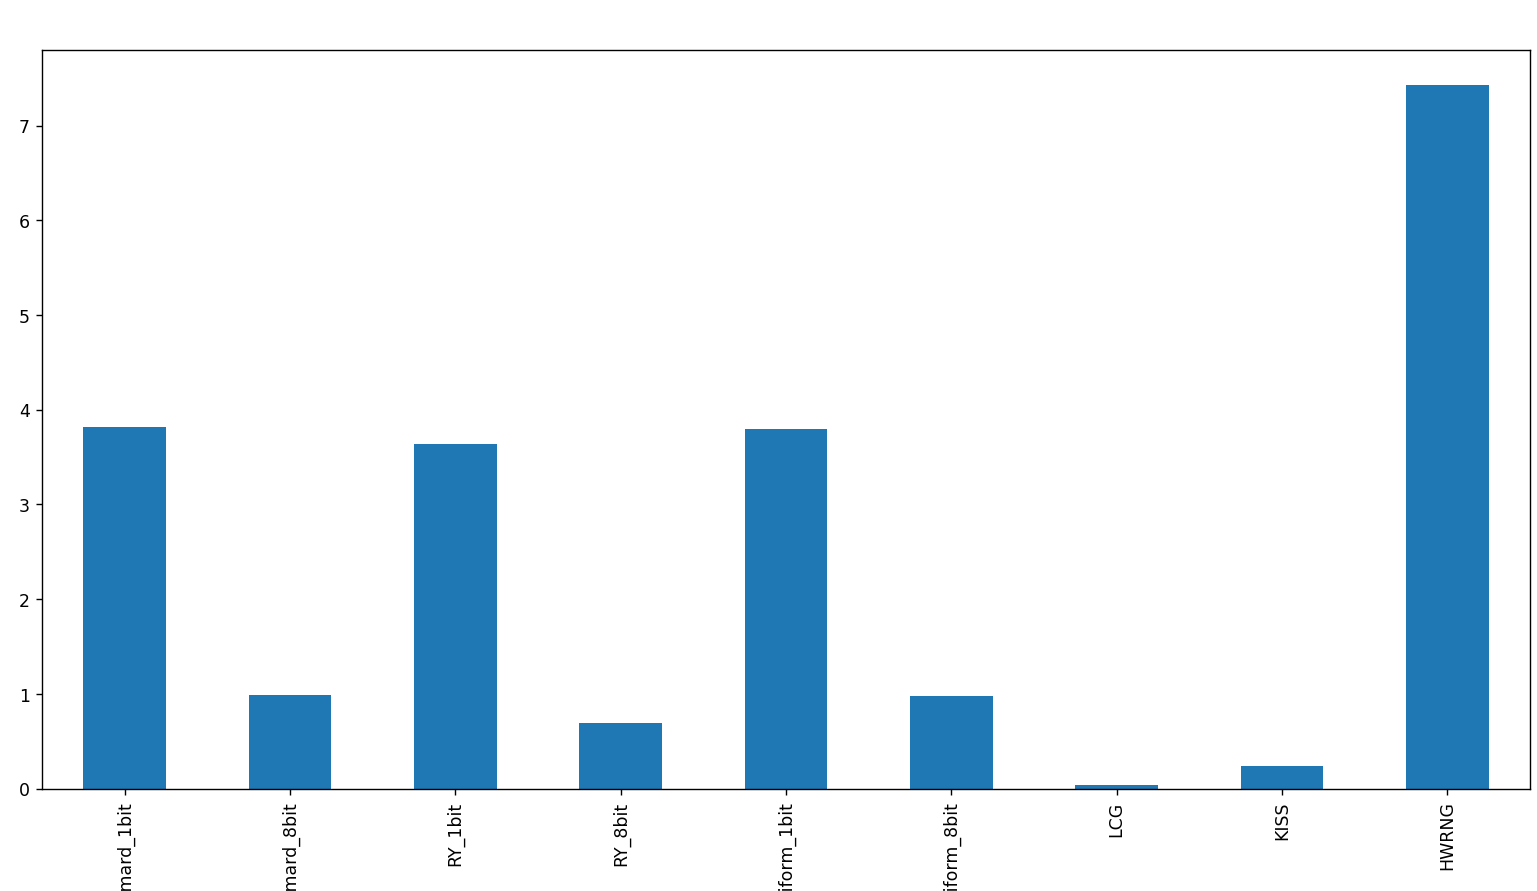
\includegraphics[width=1.0\textwidth]{continut/capitol4/figuri/UniformMeanTimes.png}
    \caption{Timpii medii de execuție}
    \label{fig:UniformMeanTimes}
\end{figure}

Și, mediile în formă tabelară:

\begin{tabular}{|l|r|}
\hline
{Generator} & {Mean execution time} \\
\hline
Hadamard\_1bit &  3.816855 \\
Hadamard\_8bit &  0.984570 \\
RY\_1bit       &  3.641219 \\
RY\_8bit       &  0.688362 \\
Uniform\_1bit  &  3.795361 \\
Uniform\_8bit  &  0.982035 \\
LCG           &  0.034659 \\
KISS          &  0.240972 \\
HWRNG         &  7.424293 \\
\hline
\end{tabular}

În concluzie, generatoarele de numere pseudoaleatorii sunt clar superioare când vine vorba de performanță. Slăbiciunea principală a generatorului de numere aleatorii hardware este faptul că trebuie să citească dintr-un fișier de tip device prin intermediul sistemului de operare.

\subsection{Timpi de execuție pentru generatoarele de numere aleatorii normale}

Pentru măsurarea timpilor de execuție, am luat în considerare numai cele mai bune două metode de generare a numerelor uniforme (LCG pentru PRNG și RY8Bit pentru QRNG), trecute prin algoritmul de transformare Box-Muller, și un circuit din biblioteca qiskit.finance, NormalDistribution(8) (Normal\_8bit). Rezultatele sunt prezentate în următoarea figură:

\begin{figure}[H]
    \centering
    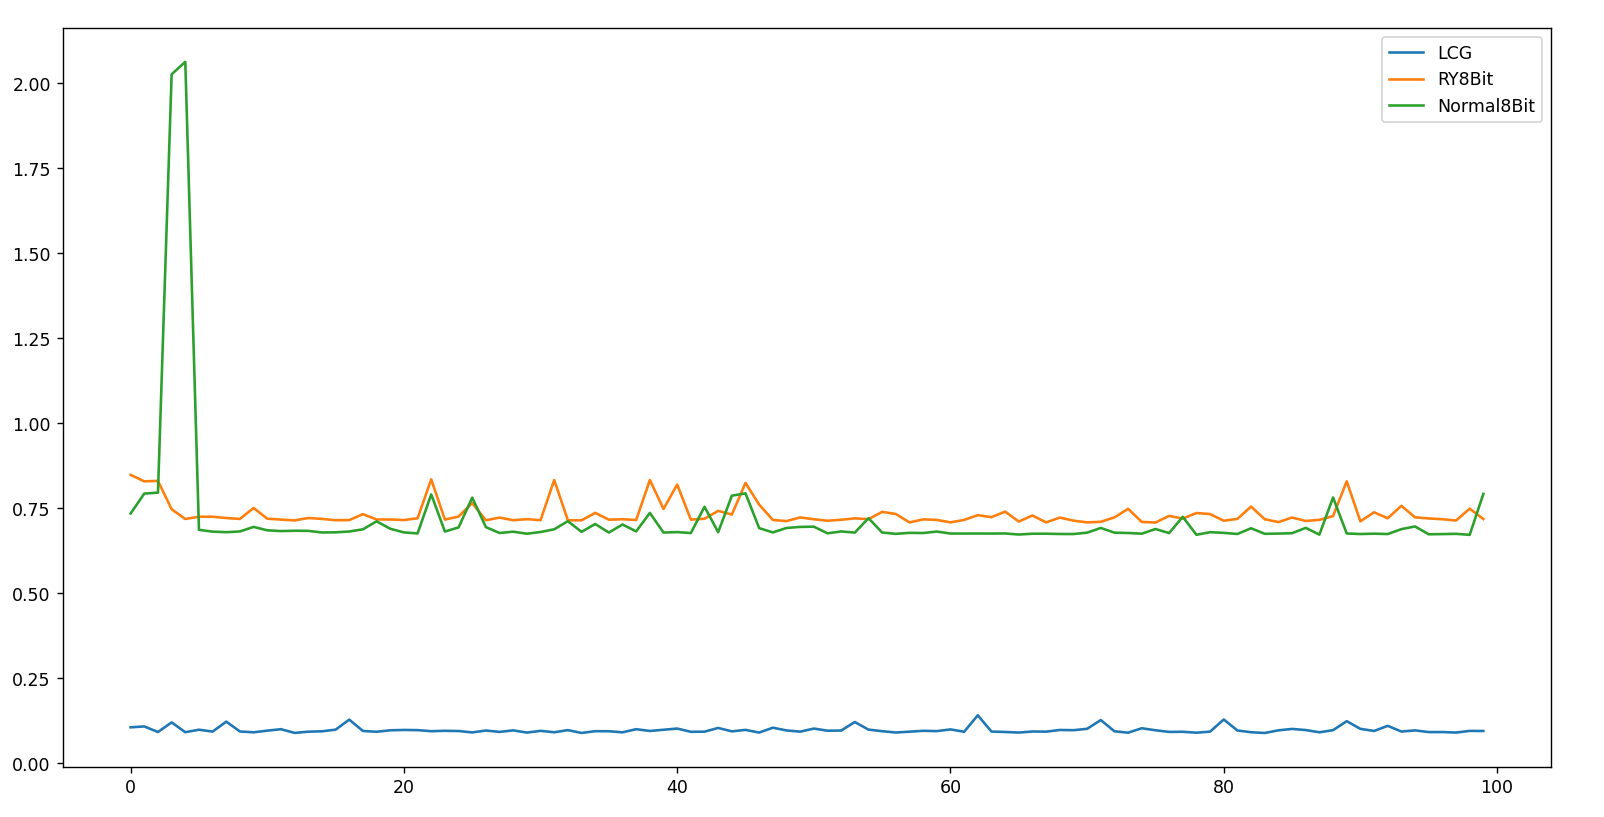
\includegraphics[width=1.0\textwidth]{continut/capitol4/figuri/NormalTimes.png}
    \caption{Timpii de execuție a metodelor de generare a numerelor pe distribuție normală}
    \label{fig:NormalTimes}
\end{figure}

Iar timpii medii de execuție:

\begin{figure}[H]
    \centering
    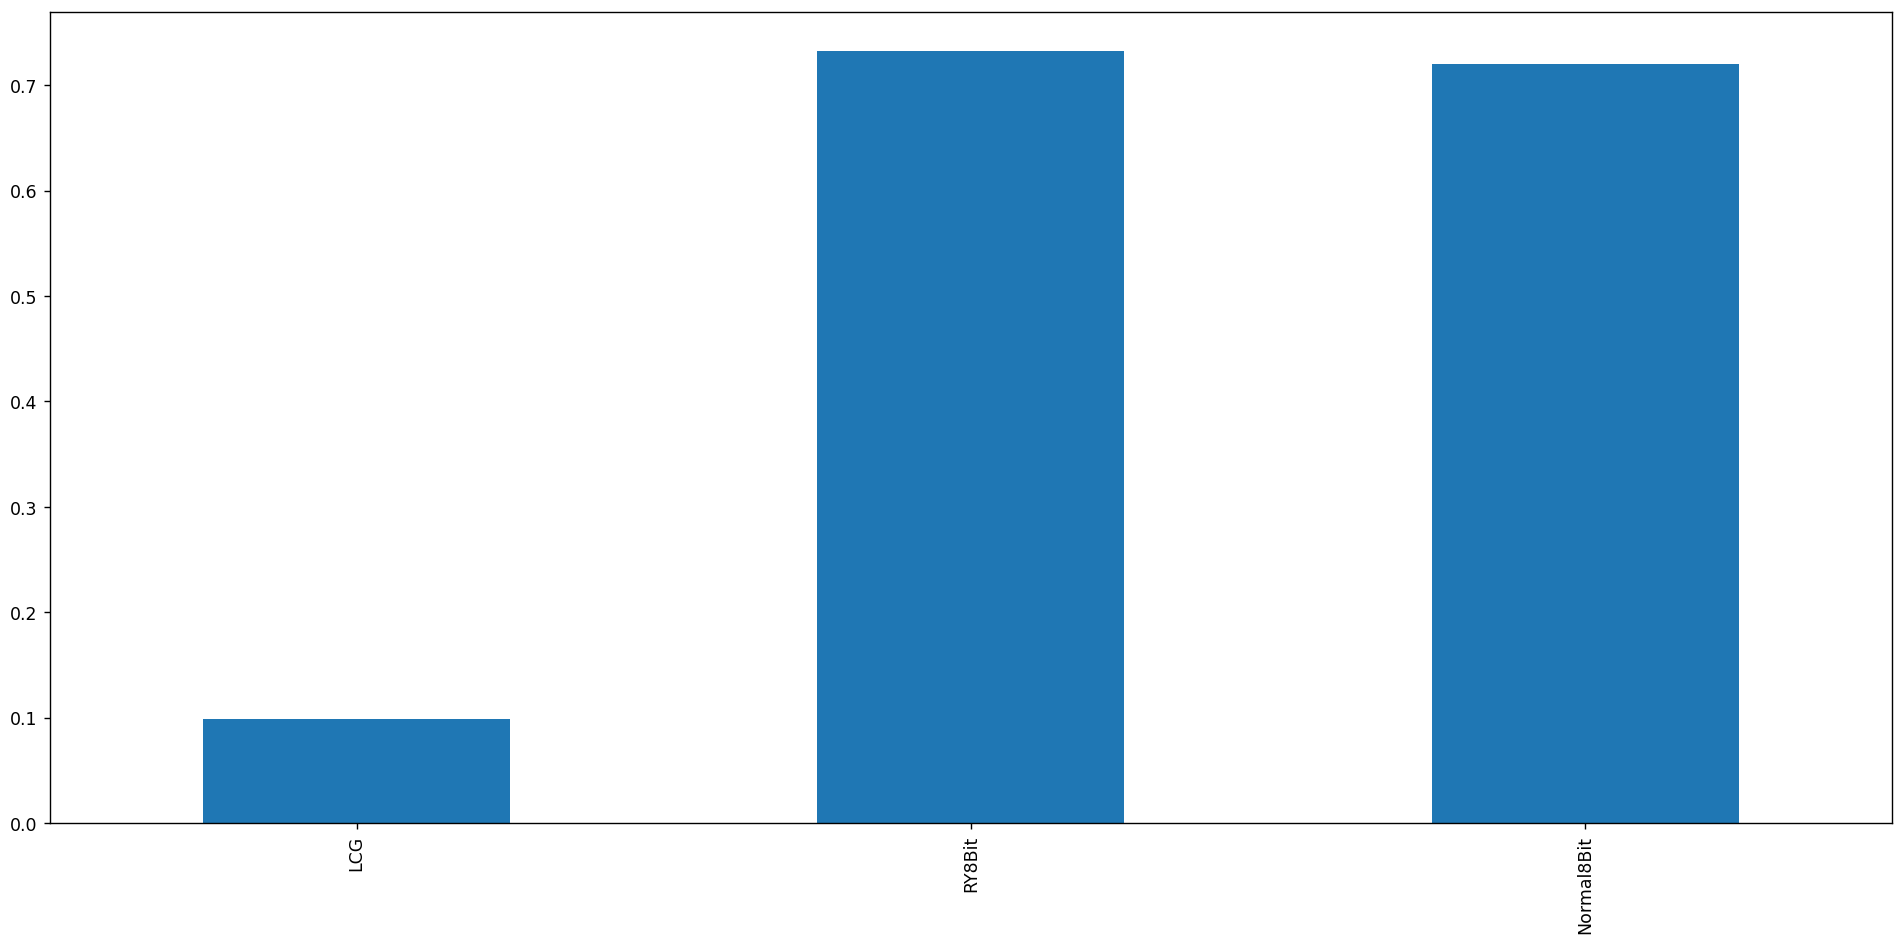
\includegraphics[width=1.0\textwidth]{continut/capitol4/figuri/NormalMeanTimes.png}
    \caption{Timpii medii de execuție a metodelor de generare a numerelor pe distribuție normală}
    \label{fig:NormalMeanTimes}
\end{figure}

Și în formă tabelară:

\begin{tabular}{|l|r|}
\hline
{Method} & {Execution time (s)} \\
\hline
LCG        &  0.098408 \\
RY8Bit     &  0.732764 \\
Normal8Bit &  0.720289 \\
\hline
\end{tabular}

În mod surprinzător, astfel, generarea unei distribuții uniforme și apoi trecerea ei prin algoritmul Box-Muller este la fel de eficient ca simularea unui circuit masiv cu sute (sau mii) de porți cuantice cum este cel din biblioteca qiskit.finance. Rămâne totuși net superioară metoda generării prin intermediul unui PRNG și apoi trecerea lui prin transformata Box-Muller.

\subsection{Rezultate statistice pentru metodele de generare a numerelor pe distribuție uniformă}

Folosind algoritmii descriși în capitolul precedent, s-au obținut următoarele rezultate statistice pentru fiecare generator în parte:

\begin{figure}[H]
    \centering
    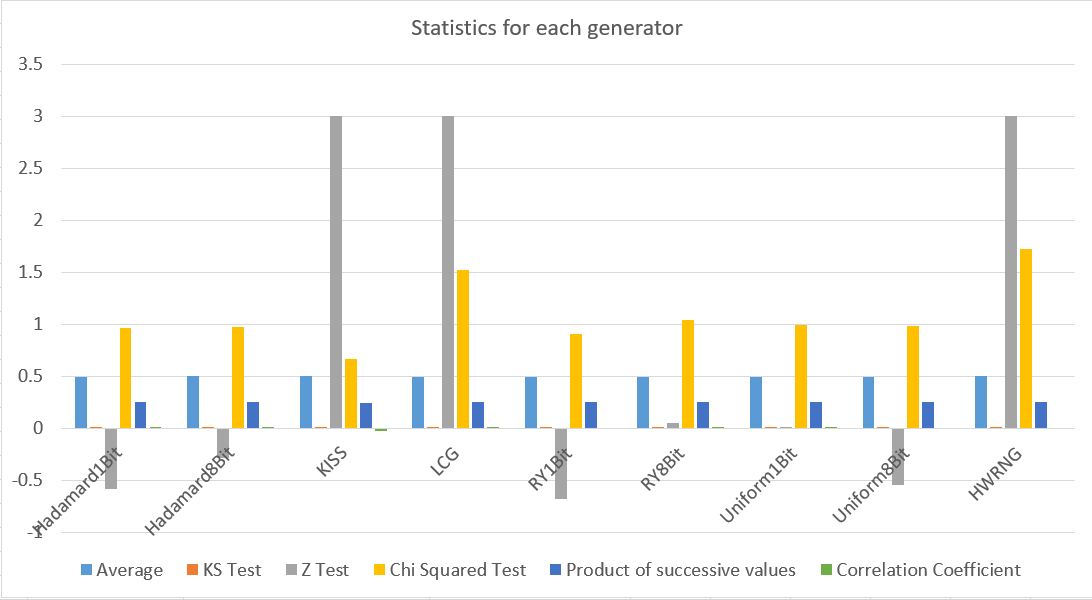
\includegraphics[width=1.0\textwidth]{continut/capitol4/figuri/ExcelStats.png}
    \caption{Grafic cu rezultatele statistice pentru fiecare generator in parte. Pentru parametrul Z, ce era mai mare de 3 a fost trecut cu 3.}
    \label{fig:AllGensExcel}
\end{figure}
Pentru rezultatele statistice pentru fiecare generator, separat, vedeți Anexa \ref{anexa1:rez_stat_gens}.

Și, aceleași date, în formă compactă, tabelară:


\resizebox{\textwidth}{!}{\begin{tabular}{lrrrrrr}
{} &     Average &   KS Test &     Z Test &  Chi Squared Test &  Product of successive values &  Correlation Coefficient \\
Generator    &             &           &            &                   &                               &                          \\
Hadamard1Bit &  127.496992 &  0.005188 &  -0.587560 &          0.966431 &                      0.249991 &                 0.000022 \\
Hadamard8Bit &  127.516155 &  0.005164 &  -0.286427 &          0.973945 &                      0.250095 &                 0.000371 \\
KISS         &  127.513699 &  0.002387 &  22.360806 &          0.670898 &                      0.247978 &                -0.024904 \\
LCG          &  127.500722 &  0.004561 &  14.824707 &          1.523027 &                      0.250025 &                 0.000256 \\
RY1Bit       &  127.491343 &  0.005140 &  -0.677467 &          0.904976 &                      0.249955 &                -0.000140 \\
RY8Bit       &  127.484699 &  0.005315 &   0.047545 &          1.043850 &                      0.249963 &                 0.000257 \\
Uniform1Bit  &  127.486854 &  0.005130 &   0.002518 &          0.994505 &                      0.249975 &                 0.000304 \\
Uniform8Bit  &  127.495929 &  0.005124 &  -0.548151 &          0.988518 &                      0.249960 &                -0.000296 \\
HWRNG &  127.823104 &  0.004794 &  16.531762 &          1.722331 &                      0.250807 &                -0.005564 \\
\end{tabular}}

Motivul pentru care testul Z dă valori atât de distribuite este din cauză că este de tip two-tailed; dacă generatorul are tendința să aibe valori atât mai mari decât (+)Z critic, cât și mai mici decât (-)Z critic, atunci media ar trebui să fie aproape 0. Dacă are tendința numai spre o coadă, atunci trebuie să fie o valoare oarecum extremă. Valorile între [-2.5, 2.5], fără valorile apropriate de 0, sunt cele rele.


